\begingroup
\begin{figure}[!htb]
    % \setArraystrech{1.5}
    \centering
    \setlength\tabcolsep{0pt}
    \begin{tabular*}{0.99\textwidth}{ c c c c c }
        Target (256px) & ImNRF (256px) & ExCol (256px) & ExVA (256px) & ExBF (64px) \\
        %%%%% GUITARS %%%%%
        \setlength\tabcolsep{0pt}
        \begin{tabular}{cc}
            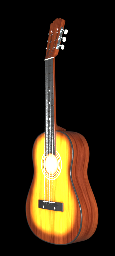
\includegraphics[width=0.095\textwidth]{figures/results/col_set/guitar0_targ_256px.png} & 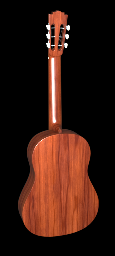
\includegraphics[width=0.095\textwidth]{figures/results/col_set/guitar8_targ_256px.png}
        \end{tabular}
        &
        \setlength\tabcolsep{0pt}
        \begin{tabular}{cc}
            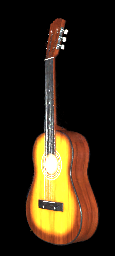
\includegraphics[width=0.095\textwidth]{figures/results/col_set/guitar0_imnf_150k.png} & 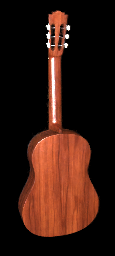
\includegraphics[width=0.095\textwidth]{figures/results/col_set/guitar8_imnf_150k.png}
        \end{tabular} 
        &
        \setlength\tabcolsep{0pt}
        \begin{tabular}{cc}
            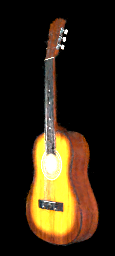
\includegraphics[width=0.095\textwidth]{figures/results/col_set/guitar0_excol_150k.png} & 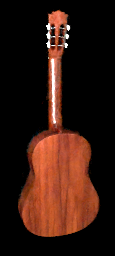
\includegraphics[width=0.095\textwidth]{figures/results/col_set/guitar8_excol_150k.png}
        \end{tabular}
        &
        \setlength\tabcolsep{0pt}
        \begin{tabular}{cc}
            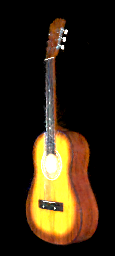
\includegraphics[width=0.095\textwidth]{figures/results/col_set/guitar0_exva_132k.png} & 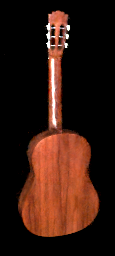
\includegraphics[width=0.095\textwidth]{figures/results/col_set/guitar8_exva_132k.png}
        \end{tabular}
        &
        \setlength\tabcolsep{0pt}
        \begin{tabular}{cc}
            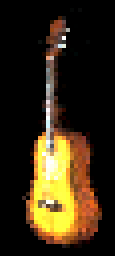
\includegraphics[width=0.095\textwidth]{figures/results/col_set/guitar0_exbf_32k.png} & 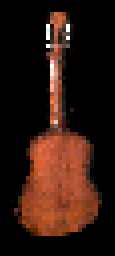
\includegraphics[width=0.095\textwidth]{figures/results/col_set/guitar8_exbf_32k.png}
        \end{tabular} \\[-5pt]
        & 150k & 150k & 150k & 30k \\
        
        
        %%%%% ROCKET %%%%%
        \setlength\tabcolsep{0pt}
        \begin{tabular}{cc}
            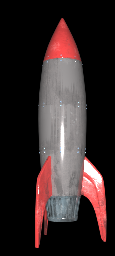
\includegraphics[width=0.095\textwidth]{figures/results/col_set/rocket0_targ_256px.png} & 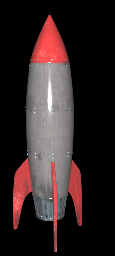
\includegraphics[width=0.095\textwidth]{figures/results/col_set/rocket4_targ_256px.png}
        \end{tabular}
        &
        \setlength\tabcolsep{0pt}
        \begin{tabular}{cc}
            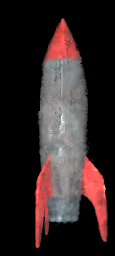
\includegraphics[width=0.095\textwidth]{figures/results/col_set/rocket0_imnf_44k.png} & 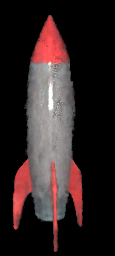
\includegraphics[width=0.095\textwidth]{figures/results/col_set/rocket4_imnf_44k.png}
        \end{tabular}
        &
        \setlength\tabcolsep{0pt}
        \begin{tabular}{cc}
            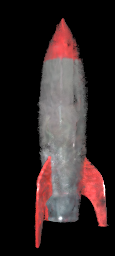
\includegraphics[width=0.095\textwidth]{figures/results/col_set/rocket0_excol_150k.png} & 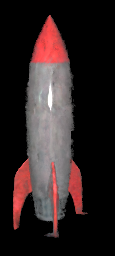
\includegraphics[width=0.095\textwidth]{figures/results/col_set/rocket4_excol_150k.png}
        \end{tabular}
        &
        \setlength\tabcolsep{0pt}
        \begin{tabular}{cc}
            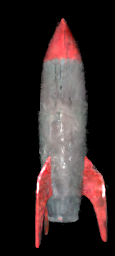
\includegraphics[width=0.095\textwidth]{figures/results/col_set/rocket0_exva_150k.png} & 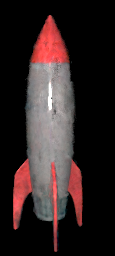
\includegraphics[width=0.095\textwidth]{figures/results/col_set/rocket4_exva_150k.png}
        \end{tabular}
        &
        \setlength\tabcolsep{0pt}
        \begin{tabular}{cc}
            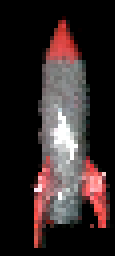
\includegraphics[width=0.095\textwidth]{figures/results/col_set/rocket0_exbf_52k.png} & 
\includegraphics[width=0.095\textwidth]{figures/results/col_set/rocket4_exbf_52k.png}
        \end{tabular} \\[-5pt]
        & 45k & 150k & 150k & 50k \\
        
        %%%%% LEGO1 %%%%%
        \begin{tabular}{cc}
            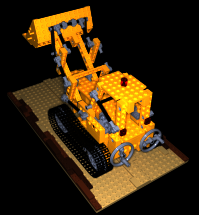
\includegraphics[width=0.19\textwidth]{figures/results/col_set/lego9_targ_256px.png} \\[-6pt]
            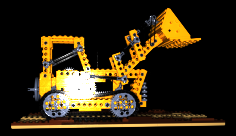
\includegraphics[width=0.19\textwidth]{figures/results/col_set/lego1_targ_256px.png}
        \end{tabular}
        &
        \begin{tabular}{cc}
            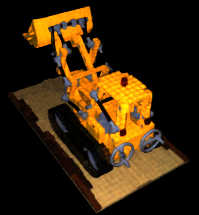
\includegraphics[width=0.19\textwidth]{figures/results/col_set/lego9_imnf_57k.png} \\[-6pt]
            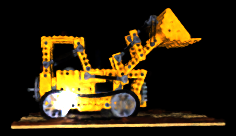
\includegraphics[width=0.19\textwidth]{figures/results/col_set/lego1_imnf_57k.png}
        \end{tabular}
        &
        \begin{tabular}{cc}
            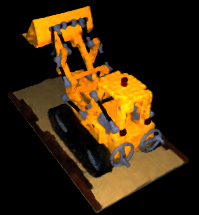
\includegraphics[width=0.19\textwidth]{figures/results/col_set/lego9_excol_57k.png} \\[-6pt]
            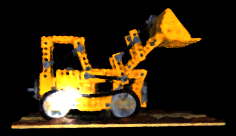
\includegraphics[width=0.19\textwidth]{figures/results/col_set/lego1_excol_57k.png}
        \end{tabular}
        &
        \begin{tabular}{cc}
            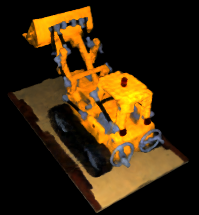
\includegraphics[width=0.19\textwidth]{figures/results/col_set/lego9_exva_51k.png} \\[-6pt]
            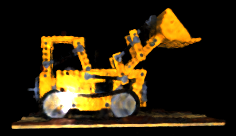
\includegraphics[width=0.19\textwidth]{figures/results/col_set/lego1_exva_51k.png}
        \end{tabular}
        &
        \begin{tabular}{cc}
            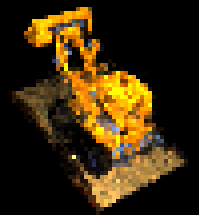
\includegraphics[width=0.19\textwidth]{figures/results/col_set/lego9_exbf_62k_voxeldefect.png} \\[-6pt]
            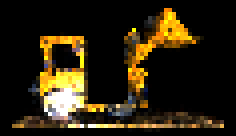
\includegraphics[width=0.19\textwidth]{figures/results/col_set/lego1_exbf_62k_voxeldefect.png}
        \end{tabular} \\[-5pt]
        & 50k & 50k & 50k & 50k \\
        
        %%%%% HOTDOG %%%%%
        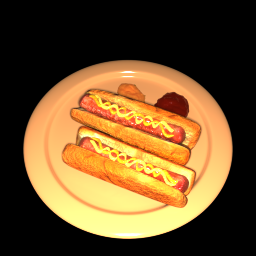
\includegraphics[width=0.19\textwidth]{figures/results/col_set/hotdog2_targ_256px.png}
        &
        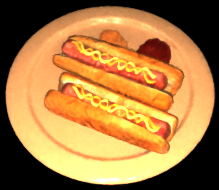
\includegraphics[width=0.19\textwidth]{figures/results/col_set/hotdog2_imnf_57k.png}
        &
        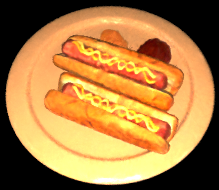
\includegraphics[width=0.19\textwidth]{figures/results/col_set/hotdog2_excol_150k.png}
        &
        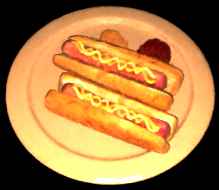
\includegraphics[width=0.19\textwidth]{figures/results/col_set/hotdog2_exva_67k.png}
        &
        
\includegraphics[width=0.19\textwidth]{figures/results/col_set/hotdog2_exbf_68k.png}
        \\ [-5pt]
        & 60k & 70k & 70k & 70k \\
        

    \end{tabular*}
    \caption{The overview of some novel view synthesis results achieved with our methods trained on colocated light setting datasets.
    Columns correspond to the schemes that have been used to obtain results.
    The number of training iterations is denoted below each result to have better understanding about model convergence.
    \textit{ExCol} and \textit{ExVA} schemes have been processed with 256px images
    while \textit{ExBF} was only trained on 64px images due to hardware limitations.
    The \textit{ExCol} and \textit{ExVA} methods generally produce similar results.
    The colocated scheme is able to reproduce fine details slightly better.
    \textit{ExBF} handles poorly geometry of Lego and Hotdog datasets,
    which results in some lacking parts of the scene
    (corresponding voxels have been pruned).
    The \textit{ExBF} are generally underfitted as training is very slow and is hard in terms of hardware.
    \im{REVIEW ImNF: waiting for results from guitar (u4103) and hotdog (u4108) in 256px}}
    \label{tab:coloc_allresults}
\end{figure}
\endgroup